\documentclass[11pt]{article}
\usepackage[margin=1in]{geometry}
\usepackage{amsmath,amssymb}
\usepackage{booktabs,longtable}
\usepackage{graphicx}
\usepackage[hidelinks]{hyperref}
\usepackage[T1]{fontenc}
\usepackage{lmodern}
\usepackage{microtype}
\emergencystretch=2em
\usepackage{xcolor}
\usepackage{natbib}
\bibliographystyle{plainnat}

% Every number in this paper is generated from the study ledger by
% `probatio study analyze`; do not type results by hand.
% generated by probatio study analyze; do not edit
\newcommand{\NumRuns}{273}
\newcommand{\NumRunErrors}{0}
\newcommand{\NumProblems}{43}
\newcommand{\NumCalibration}{28}
\newcommand{\NumUnscored}{10}
\newcommand{\NumPostHoc}{10}
\newcommand{\PostHocReached}{7}
\newcommand{\PostHocExhaustiveShort}{3}
\newcommand{\NumOpenTargets}{5}
\newcommand{\NumCandidatesChecked}{83{,}053{,}298}
\newcommand{\CalibReached}{19}
\newcommand{\AnnealSuccess}{42}
\newcommand{\AnnealRuns}{84}
\newcommand{\RandomSuccess}{24}
\newcommand{\RandomRuns}{84}
\newcommand{\NumCandidateNew}{0}
\newcommand{\OpenBelow}{5}
\newcommand{\LincodeRandomSuccess}{9}
\newcommand{\LincodeRandomRuns}{21}
\newcommand{\LincodeAnnealSuccess}{12}
\newcommand{\LincodeAnnealRuns}{21}
\newcommand{\CapsetRandomSuccess}{6}
\newcommand{\CapsetRandomRuns}{12}
\newcommand{\CapsetAnnealSuccess}{6}
\newcommand{\CapsetAnnealRuns}{12}
\newcommand{\QecRandomSuccess}{3}
\newcommand{\QecRandomRuns}{3}
\newcommand{\QecAnnealSuccess}{3}
\newcommand{\QecAnnealRuns}{3}
\newcommand{\QecExhaustiveSuccess}{1}
\newcommand{\QecExhaustiveRuns}{1}
\newcommand{\GolombRandomSuccess}{6}
\newcommand{\GolombRandomRuns}{21}
\newcommand{\GolombAnnealSuccess}{6}
\newcommand{\GolombAnnealRuns}{21}
\newcommand{\GolombExhaustiveSuccess}{6}
\newcommand{\GolombExhaustiveRuns}{6}
\newcommand{\SpreadRandomSuccess}{0}
\newcommand{\SpreadRandomRuns}{27}
\newcommand{\SpreadAnnealSuccess}{15}
\newcommand{\SpreadAnnealRuns}{27}
\newcommand{\GolombValidSix}{6.23\%}
\newcommand{\GolombValidSeven}{0.773\%}
\newcommand{\GolombValidEight}{0.0419\%}
\newcommand{\GolombValidNine}{0.001\%}
\newcommand{\GolombValidTen}{0\%}
\newcommand{\GolombValidEleven}{0\%}
\newcommand{\GolombValidTwelve}{0\%}
\newcommand{\GolombNoValid}{17}
\newcommand{\GolombHeuristicRuns}{42}
\newcommand{\ExhaustiveComplete}{15}
\newcommand{\ExhaustiveMaxSeconds}{874}

\newcommand{\pending}[1]{\textcolor{gray}{[Pending: #1]}}

\title{Exact verification as ground truth for machine-assisted mathematical discovery:\\
a pre-registered study with \textsc{Probatio}}
\author{Vasilios Venegas\\\small Independent researcher}
\date{Preprint, version 1 (classical arms), 1 November 2026}

\begin{document}
\maketitle

\begin{abstract}
Large language models and program-search agents now produce candidate mathematical
objects faster than people can check them, and the results that hold up rest on an
independent checker rather than on the generator. We present \textsc{Probatio}, an open
system in which every proposer is untrusted and every claim is re-derived by a small exact
checker, recorded as a content-addressed certificate in a hash-chained ledger, and
re-checkable by a second implementation in the reader's browser. We report the classical
arms of a pre-registered study over \NumProblems{} problems in five families (cyclic
quantum stabilizer codes, Golomb rulers, cap sets, binary linear codes and point spreading
in the unit square): \NumRuns{} runs, \NumCandidatesChecked{} exactly checked candidates and
\NumRunErrors{} run errors. Of the \NumCalibration{} scored calibration problems, the best
certified value reached the reference on \CalibReached{}. Simulated annealing succeeded in
\AnnealSuccess{}/\AnnealRuns{} calibration runs and random sampling in
\RandomSuccess{}/\RandomRuns{}; the difference is concentrated in point spreading
(\SpreadAnnealSuccess{}/\SpreadAnnealRuns{} against \SpreadRandomSuccess{}/\SpreadRandomRuns{}).
The validity of unconstrained random Golomb-ruler proposals falls from \GolombValidSix{} at
six marks to \GolombValidNine{} at nine, and no heuristic run found a valid ruler at ten or
more marks, which illustrates why exact checking, not proposal volume, is the binding
constraint. All \NumOpenTargets{} open targets remain below the recorded best values, and no
candidate record was found. In an exploratory comparison, exhaustive search shows that
codes generated by the cyclic shifts of a single Pauli operator fall short of the
general stabilizer-code optimum for $[[n,1]]$ at $n = 6, 11, 12$. The AI arms are fixed in
the frozen protocol and will be reported in a second version.
\end{abstract}

\section{Introduction}
Recent systems have produced new mathematics by pairing a generator with a verifier:
FunSearch evolved programs that output larger cap sets~\citep{funsearch2024},
AlphaEvolve and related work improved constructions across dozens of problems
\citep{alphaevolve2025,georgiev2025}, and Lean-based agents have settled open Erdős
problems~\citep{tsoukalas2026}. In each case correctness comes from the checker, not
the model. This paper makes that division explicit and measurable. We ask four
questions: how often proposals from each search method are actually valid when checked
exactly (RQ1); how often each method reaches known optima (RQ2); at what cost (RQ3);
and whether any method beats a recorded best value (RQ4).

Our contributions are: (i) an open implementation of the propose--certify--record loop
with a deliberately small trusted computing base; (ii) a pre-registered protocol whose
hash is the first entry of the study ledger, so the design cannot change after results
arrive; (iii) a benchmark of \NumProblems{} problems with cited reference values; and
(iv) baseline results for classical search, against which AI proposers will be measured.

\section{System}
\paragraph{Trust model.} Proposers (exhaustive enumeration, simulated annealing, random
sampling, language-model proposals and model-written programs) are untrusted. Their
output is data for a checker. Checkers recompute every quantity from the raw candidate
using exact integer, finite-field or rational arithmetic (trust level T2) or a proof
kernel (T1, Lean~4~\citep{lean4}).

\paragraph{Checkers.} \emph{Stabilizer codes:} commutation and GF(2) rank in the binary
symplectic representation give $k = n - \operatorname{rank}[X|Z]$; the distance
$d = \min\{\operatorname{wt}(P) : P \in N(S)\setminus S\}$ is found by exhaustive search in
order of weight~\citep{gottesman1997,crss1998}. \emph{Binary linear codes:} rank and full
enumeration of the $2^k$ codewords give $d$ and $A_d$ exactly. \emph{Cap sets:} for every
pair $a \ne b$ the third point $-(a+b) \bmod 3$ must be absent. \emph{Point spreading:}
coordinates are parsed as exact rationals and the minimum squared distance is computed
exactly. \emph{Golomb rulers:} pairwise differences must be distinct.

\paragraph{Assurance.} The Python checkers are cross-checked against independent naive
implementations (e.g.\ every cyclic stabilizer code with $n \le 6$, random codes with
$d \le 3$, 120 random linear codes) and against known objects: the [[5,1,3]] code, the
Steane and Shor codes, and the binary Golay codes, including their weight-enumerator
coefficients $A_7 = 253$ and $A_8 = 759$. A separate JavaScript implementation re-checks
every stored certificate; agreement is part of the test suite.

\paragraph{Sandbox and ledger.} Model-written programs run in a separate process with
resource limits, a resident-memory watchdog, a network namespace where available, and
an audit-hook guard blocking process creation, sockets, native code and writes outside a
scratch directory. Certificates are stored by SHA-256 of their canonical JSON; the ledger
links each entry to the hash of the previous one, and optional Ed25519 signatures bind
entries to an operator.

\section{Study design}
The protocol (Appendix~\ref{app:protocol}) was frozen before any study run; its hash is
ledger entry~0, and the runner refuses to execute if the protocol file changes. Classical
arms (random sampling, simulated annealing) run with seeds 1--3 and an equal 30\,s
wall-clock budget per run; exhaustive enumeration runs once where feasible. The AI arms
(direct model proposals; model-written generator programs) are specified with fixed
budgets of 30 model calls and US\$1 per run. The primary outcome is the success rate on
calibration problems; secondary outcomes are the normalised gap $|b - r|/r$, the
validity rate, checks-to-best and spend.

\section{Results (classical arms)}
Table~\ref{tab:summary} reports success rates with Wilson intervals by family and arm.
Figure~\ref{fig:success} shows the same data; Figure~\ref{fig:gap} shows the normalised
gap for every problem and Figure~\ref{fig:anytime} best-so-far curves.

\begin{table}[h]\centering\small
\begin{tabular}{llrrcrrr}
\toprule
Family & Arm & Runs & Success & 95\% CI & Med.\ gap & Valid & Checks to best\\
\midrule
Binary linear codes & anneal & 21 & 12/21 & [0.37, 0.76] & 0.000 & 1.00 & 2831\\
Binary linear codes & random & 21 & 9/21 & [0.24, 0.63] & 0.125 & 1.00 & 1558\\
Cap sets & anneal & 12 & 6/12 & [0.25, 0.75] & 0.044 & 1.00 & 350\\
Cap sets & random & 12 & 6/12 & [0.25, 0.75] & 0.056 & 1.00 & 541\\
Cyclic quantum codes & anneal & 3 & 3/3 & [0.44, 1.00] & 0.000 & 0.12 & 29\\
Cyclic quantum codes & exhaustive & 1 & 1/1 & [0.21, 1.00] & 0.000 & 0.29 & 8\\
Cyclic quantum codes & random & 3 & 3/3 & [0.44, 1.00] & 0.000 & 0.12 & 21\\
Golomb rulers & anneal & 21 & 6/21 & [0.14, 0.50] & 0.015 & 0.00 & 149964\\
Golomb rulers & exhaustive & 6 & 6/6 & [0.61, 1.00] & 0.000 & 1.00 & 1\\
Golomb rulers & random & 21 & 6/21 & [0.14, 0.50] & 0.029 & 0.00 & 357507\\
Point spreading & anneal & 27 & 15/27 & [0.37, 0.72] & 0.000 & 1.00 & 88437\\
Point spreading & random & 27 & 0/27 & [0.00, 0.12] & 0.217 & 1.00 & 83831\\
\bottomrule
\end{tabular}

\caption{Calibration problems: success rate (best value equals the reference) by family
and arm, Wilson 95\% intervals, median normalised gap, median validity rate and median
checks to best.}\label{tab:summary}
\end{table}

\begin{figure}[h]\centering
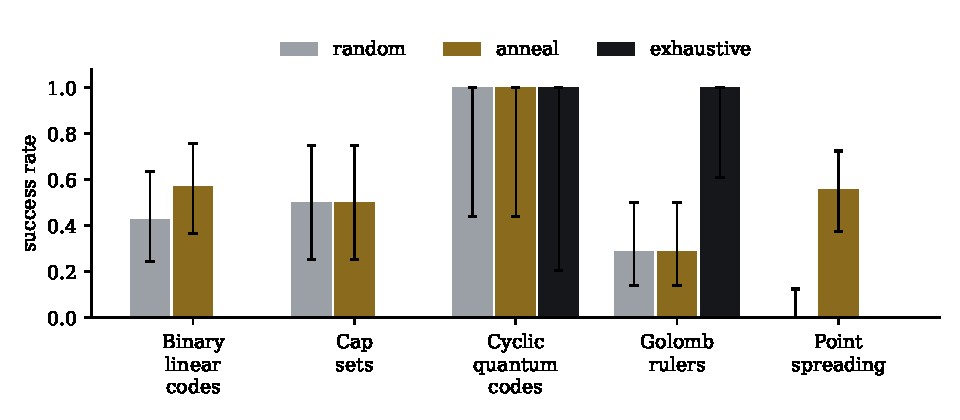
\includegraphics[width=\linewidth]{../../results/study-v1/analysis/figures/success_by_family.pdf}
\caption{Success rate on calibration problems by family and arm (Wilson 95\% intervals).}
\label{fig:success}
\end{figure}

\begin{figure}[h]\centering
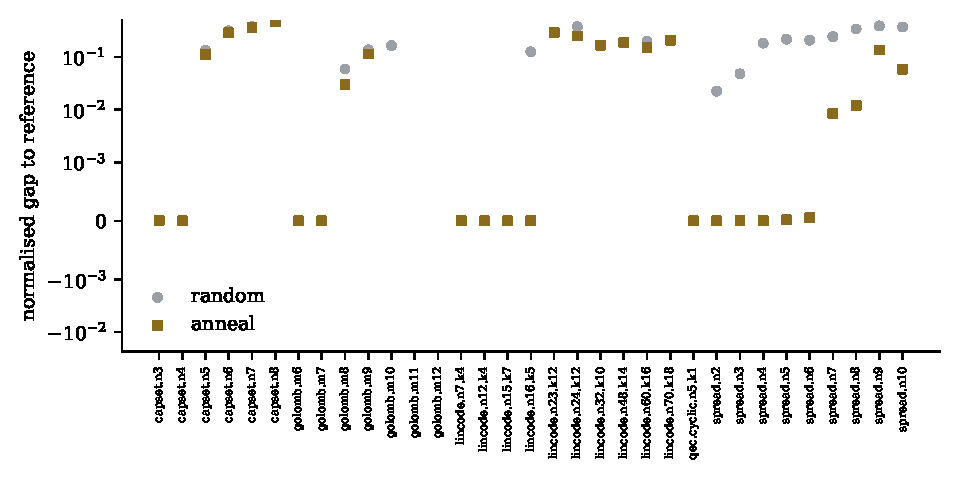
\includegraphics[width=\linewidth]{../../results/study-v1/analysis/figures/gap_by_problem.pdf}
\caption{Median normalised gap to the reference value per problem (symmetric log scale).}
\label{fig:gap}
\end{figure}

\begin{figure}[h]\centering
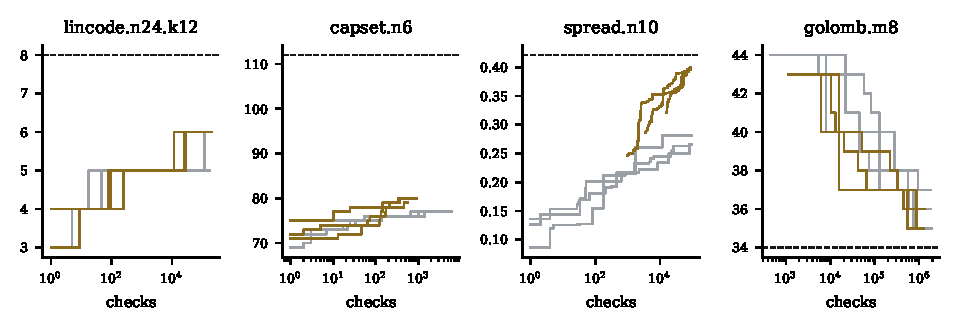
\includegraphics[width=\linewidth]{../../results/study-v1/analysis/figures/anytime.pdf}
\caption{Best-so-far value against checked candidates (log scale); dashed line: reference.}
\label{fig:anytime}
\end{figure}

\begin{table}[h]\centering\small
\begin{tabular}{lllrrrr}
\toprule
Family & A & B & A succ. & B succ. & Fisher $p$ & Holm $p$\\
\midrule
Binary linear codes & anneal & random & 12/21 & 9/21 & 0.538 & 1\\
Cap sets & anneal & random & 6/12 & 6/12 & 1 & 1\\
Cyclic quantum codes & anneal & random & 3/3 & 3/3 & 1 & 1\\
Golomb rulers & anneal & random & 6/21 & 6/21 & 1 & 1\\
Point spreading & anneal & random & 15/27 & 0/27 & $4.02\times 10^{-6}$ & $2.01\times 10^{-5}$\\
\bottomrule
\end{tabular}

\caption{Annealing versus random sampling: pooled calibration successes per family,
Fisher exact test, Holm-adjusted. Descriptive, not confirmatory.}\label{tab:tests}
\end{table}

\paragraph{RQ1 (validity).} For four families the classical proposers construct
candidates inside the valid set (systematic generator matrices, greedy cap completion,
points kept in the square), so validity is one by design. Golomb rulers are the exception:
the random and annealing proposers place marks without enforcing distinct differences,
and the median validity of random proposals falls from \GolombValidSix{} ($m=6$) to
\GolombValidSeven{} ($m=7$), \GolombValidEight{} ($m=8$) and \GolombValidNine{} ($m=9$).
In \GolombNoValid{} of \GolombHeuristicRuns{} heuristic Golomb runs no valid ruler was
found at all, all of them at $m \ge 10$, while exhaustive branch-and-bound certified the
optimum for every $m \le 11$. Cyclic stabilizer codes behave similarly: most random seeds do
not commute with their own shifts or do not give $k=1$ (Table~\ref{tab:summary}). These
rates are the baseline against which model proposals will be measured.
\pending{AI-arm validity rates.}

\paragraph{RQ2 (reaching known optima).} Of the \NumCalibration{} scored calibration
problems, \CalibReached{} were reached by at least one arm. Failures are systematic, not
noise: the binary Golay codes $[23,12,7]$ and $[24,12,8]$ and the $[32,10,12]$ code, cap sets
for $n \ge 5$ and point spreading for $n \ge 8$ were not reached by either heuristic in
30\,s. Exhaustive search was the only method that certified Golomb optima beyond $m=7$
(\ExhaustiveComplete{} complete enumerations, the longest \ExhaustiveMaxSeconds{}\,s).

\paragraph{Annealing against random sampling.} Pooled per family
(Table~\ref{tab:tests}), annealing and random sampling are indistinguishable on linear
codes, cap sets, cyclic codes and Golomb rulers. Point spreading is the only family with a
clear difference (\SpreadAnnealSuccess{}/\SpreadAnnealRuns{} against
\SpreadRandomSuccess{}/\SpreadRandomRuns{}; Holm-adjusted $p$ in Table~\ref{tab:tests}),
as expected for a continuous problem where local moves exploit geometry. These tests are
descriptive and were not the primary hypothesis.

\paragraph{RQ4 (discovery).} On the \NumOpenTargets{} open targets (cap sets in dimension 7
and 8; linear codes $[48,14]$, $[60,16]$ and $[70,18]$), the best certified values remain
below the recorded best known values (\OpenBelow{} of \NumOpenTargets{}); there are
\NumCandidateNew{} candidate records. Simple classical baselines do not reach the frontier
of these tables, which is the expected outcome and the reason the AI arms are measured
against them.

\paragraph{Exploratory: single-generator cyclic codes.} The \NumUnscored{} cyclic-code
problems with $n = 6$--$15$ had no recorded reference when the protocol was frozen, so
they are excluded from success rates (a clarification recorded in the study ledger before
the write-up). After the runs, we retrieved the optimal distance of general $[[n,1]]$
stabilizer codes from codetables.de~\citep{codetables}. Table~\ref{tab:posthoc} compares it
with the best certified code whose stabilizer is generated by the $n$ cyclic shifts of a
single Pauli operator. Enumeration of this class was complete for $n \le 13$ and was
repeated without symmetry reduction for $n \le 11$ by an independent script, with identical
results. The class attains the general optimum for $n = 7$--$10$ and $13$ but falls short at
$n = 6$, $11$ and $12$. This statement concerns one construction class only; cyclic codes
generated by several operators are outside it, and we make no claim of novelty.

\begin{table}[h]\centering\small
\begin{tabular}{lrcrc}
\toprule
Problem & Best certified & Exhaustive & Post-hoc ref. & Reached\\
\midrule
\texttt{qec.cyclic.n6.k1} & 2 & yes & 3 & no\\
\texttt{qec.cyclic.n7.k1} & 3 & yes & 3 & yes\\
\texttt{qec.cyclic.n8.k1} & 3 & yes & 3 & yes\\
\texttt{qec.cyclic.n9.k1} & 3 & yes & 3 & yes\\
\texttt{qec.cyclic.n10.k1} & 4 & yes & 4 & yes\\
\texttt{qec.cyclic.n11.k1} & 3 & yes & 5 & no\\
\texttt{qec.cyclic.n12.k1} & 4 & yes & 5 & no\\
\texttt{qec.cyclic.n13.k1} & 5 & yes & 5 & yes\\
\texttt{qec.cyclic.n14.k1} & 5 & no & 5 & yes\\
\texttt{qec.cyclic.n15.k1} & 5 & no & 5 & yes\\
\bottomrule
\end{tabular}

\caption{Exploratory. Best certified distance among $[[n,1]]$ codes generated by the cyclic
shifts of one Pauli operator, against the optimum over all stabilizer codes
(codetables.de, retrieved 2026-11-01, after the study ran).}\label{tab:posthoc}
\end{table}

\section{Discussion and limitations}
The value of this version is the infrastructure and the baseline, not new mathematics.
Every number above is backed by a certificate that a reader can re-check independently, and
the protocol fixes in advance how AI proposers will be compared. Three limitations matter.
First, the classical baselines are intentionally simple; stronger domain-specific methods
(structured cap constructions~\citep{edel2004}, algebraic code constructions,
interval-verified packing optimisation~\citep{markot2005}) would raise the bar. Second,
wall-clock budgets make results depend on hardware and concurrent load; candidate counts
are reported for this reason. Third, point-spreading optima are irrational, so rational
candidates can only approach them, and success there means agreement within $10^{-4}$.
Verification establishes correctness, not novelty: any future record will be reported only
after the literature review specified in the protocol. Formal-proof problems are excluded
from scoring until a Lean toolchain is part of the reproducibility image.

\section{Reproducibility}
The repository contains the protocol, problem specifications, the complete ledger and
certificates. \texttt{scripts/reproduce.sh} re-runs the test suite, re-verifies every
certificate, audits the ledger and regenerates every table, figure and number in this
paper; \texttt{probatio study run} re-executes the study from scratch.

\paragraph{Use of AI assistance.} The software and this manuscript were developed with
the assistance of an AI model (Claude, Anthropic); all results are produced and checked by
the deterministic code described here.

\bibliography{refs}

\appendix
\section{Per-problem results}
\small
\begin{longtable}{llrrrll}
\toprule
Problem & Role & Ref. & Upper & Best & Arm & Status\\
\midrule
\endhead
\texttt{capset.n3} & calibration & 9 & — & 9 & random & matches-known\\
\texttt{capset.n4} & calibration & 20 & — & 20 & random & matches-known\\
\texttt{capset.n5} & calibration & 45 & — & 41 & anneal & below-known\\
\texttt{capset.n6} & calibration & 112 & — & 80 & anneal & below-known\\
\texttt{capset.n7} & open-target & 236 & — & 153 & anneal & below-known\\
\texttt{capset.n8} & open-target & 512 & — & 277 & anneal & below-known\\
\texttt{golomb.m6} & calibration & 17 & — & 17 & exhaustive & matches-known\\
\texttt{golomb.m7} & calibration & 25 & — & 25 & exhaustive & matches-known\\
\texttt{golomb.m8} & calibration & 34 & — & 34 & exhaustive & matches-known\\
\texttt{golomb.m9} & calibration & 44 & — & 44 & exhaustive & matches-known\\
\texttt{golomb.m10} & calibration & 55 & — & 55 & exhaustive & matches-known\\
\texttt{golomb.m11} & calibration & 72 & — & 72 & exhaustive & matches-known\\
\texttt{golomb.m12} & calibration & 85 & — & — & --- & no result\\
\texttt{lincode.n7.k4} & calibration & 3 & 3 & 3 & random & matches-known\\
\texttt{lincode.n12.k4} & calibration & 6 & 6 & 6 & random & matches-known\\
\texttt{lincode.n15.k7} & calibration & 5 & 5 & 5 & random & matches-known\\
\texttt{lincode.n16.k5} & calibration & 8 & 8 & 8 & anneal & matches-known\\
\texttt{lincode.n23.k12} & calibration & 7 & 7 & 5 & random & below-known\\
\texttt{lincode.n24.k12} & calibration & 8 & 8 & 6 & random & below-known\\
\texttt{lincode.n32.k10} & calibration & 12 & 12 & 10 & random & below-known\\
\texttt{lincode.n48.k14} & open-target & 16 & 17 & 14 & anneal & below-known\\
\texttt{lincode.n60.k16} & open-target & 20 & 22 & 17 & anneal & below-known\\
\texttt{lincode.n70.k18} & open-target & 24 & 26 & 19 & random & below-known\\
\texttt{qec.cyclic.n5.k1} & calibration & 3 & 3 & 3 & exhaustive & matches-known\\
\texttt{qec.cyclic.n6.k1} & calibration & — & 3 & 2 & exhaustive & no-recorded-bound\\
\texttt{qec.cyclic.n7.k1} & calibration & — & 4 & 3 & exhaustive & no-recorded-bound\\
\texttt{qec.cyclic.n8.k1} & calibration & — & 4 & 3 & exhaustive & no-recorded-bound\\
\texttt{qec.cyclic.n9.k1} & calibration & — & 5 & 3 & exhaustive & no-recorded-bound\\
\texttt{qec.cyclic.n10.k1} & calibration & — & 5 & 4 & exhaustive & no-recorded-bound\\
\texttt{qec.cyclic.n11.k1} & calibration & — & 6 & 3 & exhaustive & no-recorded-bound\\
\texttt{qec.cyclic.n12.k1} & calibration & — & 6 & 4 & exhaustive & no-recorded-bound\\
\texttt{qec.cyclic.n13.k1} & calibration & — & 7 & 5 & exhaustive & no-recorded-bound\\
\texttt{qec.cyclic.n14.k1} & calibration & — & 7 & 5 & random & no-recorded-bound\\
\texttt{qec.cyclic.n15.k1} & calibration & — & 8 & 5 & random & no-recorded-bound\\
\texttt{spread.n2} & calibration & 1.4142 & — & 1.4142 & anneal & matches-known\\
\texttt{spread.n3} & calibration & 1.0353 & — & 1.0353 & anneal & matches-known\\
\texttt{spread.n4} & calibration & 1 & — & 1 & anneal & matches-known\\
\texttt{spread.n5} & calibration & 0.7071 & — & 0.7071 & anneal & matches-known\\
\texttt{spread.n6} & calibration & 0.6009 & — & 0.6009 & anneal & matches-known\\
\texttt{spread.n7} & calibration & 0.5359 & — & 0.5358 & anneal & matches-known\\
\texttt{spread.n8} & calibration & 0.5176 & — & 0.5116 & anneal & below-known\\
\texttt{spread.n9} & calibration & 0.5000 & — & 0.4418 & anneal & below-known\\
\texttt{spread.n10} & calibration & 0.4213 & — & 0.3994 & anneal & below-known\\
\bottomrule
\end{longtable}


\section{Protocol}\label{app:protocol}
The full pre-registered protocol is in the repository file\\
\texttt{experiments/PROTOCOL.md}. Its machine-readable form,\\
\texttt{experiments/protocol-v1.json}, is hashed into ledger entry~0. Two operator notes,
recorded in the ledger after the runs and before the write-up, document the scoring
clarification for problems without a reference and the independent cross-check of the
exhaustive cyclic-code results.
\end{document}
